\documentclass[11pt,a4paper]{article}
\usepackage[margin=21mm,top=22mm,bottom=20mm]{geometry}
\usepackage{amsmath,amssymb}
\usepackage{graphicx}
\usepackage{booktabs}
\usepackage{xltabular}
\usepackage{array}
\usepackage{xcolor}
\usepackage[most]{tcolorbox}
\usepackage{titlesec}
\usepackage{caption}
\usepackage{float}
\usepackage{fancyhdr}
\usepackage{enumitem}
\usepackage{siunitx}
\usepackage[colorlinks=true,linkcolor=black,citecolor=black,urlcolor=black]{hyperref}
\graphicspath{{/home/claude/work/sle/cryo-sle/figures/}{./}}

\definecolor{mid}{HTML}{5B6B72}
\definecolor{pale}{HTML}{EEF3F4}
\definecolor{acc}{HTML}{0D5D70}
\setlength{\parskip}{4pt}
\setlength{\parindent}{0pt}
\captionsetup{font=small,labelfont=bf}
\titleformat{\section}{\Large\bfseries\color{acc}}{\thesection}{0.6em}{}
\titleformat{\subsection}{\large\bfseries}{\thesubsection}{0.5em}{}
\titleformat{\subsubsection}{\normalsize\bfseries}{\thesubsubsection}{0.5em}{}
\setlist{itemsep=1pt,topsep=2pt}
\newcolumntype{L}{>{\raggedright\arraybackslash}X}
\newtcolorbox{idea}[1][]{colback=pale,colframe=pale,boxrule=0pt,arc=2pt,left=8pt,right=8pt,top=5pt,bottom=5pt,fontupper=\small,#1}
\newcommand{\dfus}{\Delta_{\mathrm{fus}}}
\newcommand{\aoh}{a_{\mathrm{OH}}}
\newcommand{\file}[1]{\texttt{\small #1}}

\pagestyle{fancy}\fancyhf{}
\fancyhead[L]{\footnotesize\color{mid}Cryo-SLE project handbook}
\fancyhead[R]{\footnotesize\color{mid}S. Chowdhary, 25B0347 --- CL207}
\fancyfoot[C]{\footnotesize\thepage}
\renewcommand{\headrulewidth}{0.3pt}

\begin{document}

\begin{center}
{\LARGE\bfseries Cryo-SLE project handbook}\\[6pt]
{\large The whole project from scratch: background, papers, tests, equations, code}\\[6pt]
{\normalsize Siddhant Chowdhary (25B0347) \quad CL207 Chemical Engineering Thermodynamics, IIT Bombay}\\[2pt]
{\small\color{mid}Written 30 Oct 2026. Companion to the 5-page report (\file{report/report\_final.pdf}).}
\end{center}

\begin{idea}
\textbf{How to use this handbook.} Section~1 is the story in one page. Section~2 teaches every piece of
thermodynamics the project uses, intuition first, then the equation. Section~3 lists every paper and data source
and what it was used for. Section~4 walks through every test in the order it was done, with the question, the
method, the result and the file. Section~5 summarises the results. Section~6 explains the code and how to run it
yourself. Sections~7--9 record assumptions, limitations and what is left to do.
\end{idea}

\tableofcontents
\clearpage

%======================================================================
\section{The project in one page}

\textbf{The problem.} When cells are frozen slowly, ice forms outside them first. Ice is pure water, so the salt
that was dissolved in that water stays behind in a shrinking pocket of liquid. The salt concentration rises, water
is pulled out of the cells, and cells die. This ``solution effect'' is one of the two main causes of freezing
injury \cite{mazur}. Cryoprotectants such as glycerol help by staying in the liquid with the salt and diluting it
\cite{lovelock11}, but they are toxic at high doses, so we want as little as possible.

\textbf{The thermodynamic insight.} At equilibrium, water has the same chemical potential in ice and in the liquid.
Because ice is pure, this fixes the water activity of the liquid at each temperature, whatever is dissolved in it.
A cryoprotectant cannot change that activity. It can only change how much water must freeze before the liquid
reaches it, and therefore how concentrated the salt becomes.

\textbf{The question.} Can we predict freeze concentration from thermodynamics alone, with as few fitted numbers as
possible, and use that to design cryoprotectant mixtures?

\textbf{The hypothesis.} The non-ideality of water--polyol mixtures comes from hydrogen bonds between water and
hydroxyl (--OH) groups. So one interaction constant \emph{per OH group}, fitted on one molecule (glycerol), should
predict other polyols and polyol\,+\,salt mixtures without refitting.

\textbf{What we did.}
\begin{enumerate}
\item Built the solid--liquid equilibrium (SLE) model and fitted one constant, $\aoh=-2414.9$\,J\,mol$^{-1}$ per OH,
on 19 glycerol freezing points.
\item Froze that constant and the predictions in git, then tested them blind against literature data: 11 single
solutes, two solutes at 25\,\textdegree C, and the water--glycerol--NaCl phase diagram (digitised by hand).
\item Compared against five other models: ideal solution, UNIFAC, Dortmund UNIFAC, the osmotic virial equation and
the Kleinhans--Mazur summation.
\item Diagnosed the failures (post hoc, clearly labelled).
\item Used the model to compute freeze concentration outside and inside a cell, and designed glycerol-sparing
recipes under three injury criteria from the literature.
\item Built a one-command reproducible pipeline and an interactive web tool.
\end{enumerate}

\textbf{The answer, in short.}
\begin{itemize}
\item The per-OH constant transfers to ethylene glycol and sucrose (3$\times$ and 17$\times$ better than ideal) and
gets the right sign of non-ideality, where UNIFAC gets it wrong.
\item For glycerol\,+\,salt above 30\,wt\% solute it beats both cryobiology models by about 3--5$\times$.
\item It fails for sorbitol and simple alcohols. The failure is due to the molecule (crowded OH groups), not
temperature.
\item A non-penetrating additive (sorbitol) lowers salt outside the cell but cannot lower it inside. Whether sorbitol
saves glycerol depends on which injury mechanism dominates; the model quantifies each case.
\end{itemize}

%======================================================================
\section{Background: the thermodynamics used}

Each subsection gives the intuition first and then the equation. Course references are to Sandler \cite{sandler}.

\subsection{Freezing point depression}
\textbf{Intuition.} Pure water freezes at 0\,\textdegree C. Dissolve something in it and water molecules are
``diluted'': fewer of them sit at any spot where they could join the ice, so their escaping tendency drops. You
must go colder before ice forms. More solute means colder. For dilute solutions the drop depends only on how many
solute particles there are (colligative), which is why NaCl (two ions) depresses about twice as much as glycerol per
mole.

\textbf{Equation (dilute limit).} $\Delta T_f \approx K_f\,m\,\nu$, with $K_f = RT_m^2M_w/\dfus H = 1.86$\,K\,kg\,mol$^{-1}$
for water, $m$ the molality and $\nu$ the number of particles per formula unit. The rest of this section is about
going beyond this limit.

\subsection{The equilibrium condition: equal chemical potential}
\textbf{Intuition.} At equilibrium nothing moves on average. Water molecules leave the ice for the liquid as often as
they leave the liquid for the ice. That happens when water's chemical potential (its ``escaping tendency'') is the
same in both phases.

\textbf{Equation.} $\mu_w^{\mathrm{ice}}(T,P)=\mu_w^{\mathrm{L}}(T,P,x)$. Writing the liquid with the pure
supercooled liquid as reference, $\mu_w^{\mathrm{L}}=\mu_w^{\mathrm{L},0}(T)+RT\ln(x_w\gamma_w)$, so
\begin{equation}
RT\ln(x_w\gamma_w) = \mu_w^{\mathrm{ice}}(T)-\mu_w^{\mathrm{L},0}(T) = -\dfus G(T).
\end{equation}
$x_w\gamma_w=a_w$ is the water activity. Equivalently, the fugacities are equal, $f_w^{\mathrm{ice}}=x_w\gamma_wf_w^{\mathrm{L},0}$.

\subsection{Getting $\dfus G(T)$: the heat--melt--cool path}
\textbf{Intuition.} We know melting data at 0\,\textdegree C. To get the Gibbs energy of melting at, say,
$-15$\,\textdegree C, build a path: warm the ice to 0\,\textdegree C, melt it, cool the liquid back to
$-15$\,\textdegree C. Gibbs energy is a state function, so the path doesn't matter.

\textbf{Equation.} With constant $\dfus H$ and $\Delta C_p=C_p^{\mathrm{L}}-C_p^{\mathrm{ice}}$,
\begin{equation}
\ln a_w = \ln(x_w\gamma_w) = -\frac{\dfus H}{R}\left(\frac1T-\frac1{T_m}\right)-\frac{\Delta C_p}{R}\left(\frac{T_m}{T}-1+\ln\frac{T}{T_m}\right),
\label{eq:sle}
\end{equation}
with $\dfus H=6009.5$\,J\,mol$^{-1}$, $\Delta C_p=37.9$\,J\,mol$^{-1}$\,K$^{-1}$, $T_m=273.15$\,K. This is the central
equation of the project.

\begin{idea}
\textbf{The key consequence.} The right-hand side depends only on $T$. Once ice is present, the water activity of
\emph{every} liquid in contact with it is fixed by temperature. Additives cannot change $a_w$; they change how much
water has to freeze out to reach it. A cell at osmotic equilibrium has the same $a_w$ inside, so its interior is
also fixed by $T$, and which solutes can enter the cell decides how salty the interior gets.
\end{idea}

\subsection{Activity coefficients and excess Gibbs energy}
\textbf{Intuition.} $\gamma_w$ measures how far water's escaping tendency is from ideal (Raoult). If water ``likes''
the solute more than itself (hydrogen bonds to --OH), it is held more tightly: $\gamma_w<1$, and the freezing point
drops more than ideal. If it dislikes the solute, $\gamma_w>1$ and the drop is smaller.

\textbf{Equation.} The excess Gibbs energy $G^{\mathrm{ex}}$ collects all non-ideality; activity coefficients follow
by differentiation, $RT\ln\gamma_i=(\partial nG^{\mathrm{ex}}/\partial n_i)_{T,P,n_{j\ne i}}$. The simplest model is
one-constant (two-suffix) Margules for a binary: $G^{\mathrm{ex}}/RT=\alpha x_wx_s$, giving
$\ln\gamma_w=\alpha x_s^2$.

\subsection{The per-OH model (this project)}
\textbf{Idea.} Keep only water--solute pair interactions and make each solute's interaction proportional to its
number of OH groups:
\begin{equation}
\frac{G^{\mathrm{ex}}}{RT}=x_w\sum_i\alpha_ix_i,\qquad \alpha_i=\frac{n_{\mathrm{OH},i}\,\aoh}{RT},\qquad
\ln\gamma_w=(1-x_w)\sum_i\alpha_ix_i .
\label{eq:model}
\end{equation}
One number, $\aoh$, describes every polyol. $\aoh<0$ means attraction (hydrogen bonding). The $1/T$ in $\alpha$
comes from assuming the interaction \emph{energy} is constant; Section~4.11 tests that.

\subsection{Gibbs--Duhem: a consistency check}
At fixed $T,P$, $\sum_i x_i\,d\ln\gamma_i=0$. Any $\gamma$'s derived from one $G^{\mathrm{ex}}$ satisfy it
automatically; we check it numerically (residual $\sim10^{-14}$) to catch coding errors.

\subsection{Group contribution and UNIFAC}
\textbf{Intuition.} Instead of fitting every molecule, split molecules into groups (CH$_2$, OH, \ldots) and fit
group--group interactions once on a large database. UNIFAC \cite{unifac} and its Dortmund modification \cite{dortmund}
do this, mostly from vapour--liquid data at and above room temperature. Our model is an extreme special case: one
group (OH), one interaction, fitted on freezing data. The trade-off is breadth (UNIFAC) against accuracy in one
class of molecules (ours).

\subsection{Electrolytes: the osmotic coefficient}
\textbf{Intuition.} Salt splits into ions that attract each other over long distances (Debye--H\"uckel), so NaCl is
strongly non-ideal even when dilute. It is usual to describe it with the osmotic coefficient $\phi$: the factor by
which the real water-activity lowering differs from the ideal one.

\textbf{Equation.} $\ln a_w^{\mathrm{NaCl}}=-\nu mM_w\phi(m)$ with $\nu=2$. We fit
$\phi=1-a\sqrt m/(1+\sqrt m)+bm+cm^2$ to the CRC NaCl ice line: $a,b,c=0.2602,\ 0.0523,\ 0.0061$ (RMSE 0.023\,K up to
the eutectic). The $\sqrt m$ term has the Debye--H\"uckel shape.

\subsection{Mixing rules for salt + polyol}
Three ways to predict a mixture from single-solute data:
\begin{itemize}
\item \textbf{Additive in $\ln a_w$ (ours).} $\ln a_w(\text{mix})=\ln a_w(\text{polyol part})+\ln a_w(\text{salt part})$
at the mixture's molalities. It follows from the activity framework when solutes don't interact directly.
\item \textbf{Kleinhans--Mazur summation} \cite{km}. Add the two binary freezing-point depressions at the mixture's
molalities. Works when dilute; not built on activities.
\item \textbf{Osmotic virial} \cite{elliott,zielinski}. Osmolality $\pi=\sum k_im_i+\sum_{ij}\tfrac{B_{ii}+B_{jj}}2k_im_ik_jm_j$,
with coefficients fitted per solute; $\ln a_w=-M_w\pi$.
\end{itemize}

\subsection{Freeze concentration: water balance (lever rule)}
\textbf{Intuition.} Start with a solution; cool it below its freezing point. Ice forms, taking only water. Keep
removing water until the remaining liquid's $a_w$ equals the ice value at that $T$.

\textbf{Equation.} With starting water $W_0$ and solutes $n_j$, the frozen fraction $\varphi$ solves
\begin{equation}
\ln a_w\big(\{n_j\},(1-\varphi)W_0\big)=\ln a_w^{\mathrm{ice}}(T)\quad\text{(right side from eq.~\ref{eq:sle})}.
\label{eq:balance}
\end{equation}
The unfrozen fraction is $1-\varphi$, and the salt mass fraction in the liquid follows from the mass balance.

\subsection{The cell at osmotic equilibrium}
\textbf{Intuition.} A cell membrane lets water through freely. In slow cooling, water leaves the cell until its
chemical potential inside equals outside, which equals the ice value. Glycerol also crosses (it is
``penetrating''); sorbitol and NaCl do not.

\textbf{Equation.} With the cell's own solutes $n_c$ (represented as isotonic NaCl), glycerol at the outside molality
$m_g(T)$, and cell water $W_c$:
\begin{equation}
\ln a_w\big(n_c/W_c,\ m_g(T)\big)=\ln a_w^{\mathrm{ice}}(T).
\label{eq:cell}
\end{equation}
If only sorbitol is added, the inside contains only the cell's own salts, so inside salt is exactly what it would be
in plain saline. This is Pegg's ``must penetrate'' \cite{pegg} in one line.

\subsection{Gibbs--Helmholtz: splitting the interaction into $h$ and $s$}
\textbf{Intuition.} A free energy has an energy part and an entropy part, $a=h-Ts$. Hydrogen bonds release energy
($h<0$) but also order the water around the solute ($s<0$). As $T$ rises, the $-Ts$ term (positive) grows and the net
attraction weakens. Measuring $a$ at two temperatures separates the two.

\textbf{Equation.} $a(T)=h-Ts$, so $s=-[a(T_2)-a(T_1)]/(T_2-T_1)$ and $h=a(T_1)+T_1s$.

\subsection{Eutectics (why an ice--salt bath stops at $-21$\,\textdegree C)}
Ice + NaCl + saturated brine coexist only at the NaCl--water eutectic, $-21.1$\,\textdegree C at 23.3\,wt\% NaCl. A
bath of ice and salt cannot go colder; this sets the cold limit of the proposed experiment.

%======================================================================
\section{Papers and data sources}

Every number used in the project comes from one of these sources; the data files record the page or table.

\subsection*{Data used to fit or test the model}
\begin{xltabular}{\textwidth}{@{}p{4.2cm}Lp{3.2cm}@{}}
\toprule
Source & What it contains & How we used it\\
\midrule
CRC Handbook, Internet Version 2005, pp.\ 8-58 to 8-84 \cite{crc} & Freezing points of glycerol, NaCl, ethylene glycol, mannitol, sugars, alcohols & Fit (glycerol), NaCl model, blind tests\\
Siniti, Jabrane \& L\'etoff\'e 1999 \cite{siniti} & Sorbitol--water phase diagram by DSC, 35--64\,wt\% & Blind test (concentrated sorbitol)\\
Baer \& Baldwin 1984 \cite{baer} & Cryoscope freezing points of sorbitol and sucrose, 1--11\,wt\% & Tested, then flagged ($\phi\approx1.14$ at 1\,wt\%, impossible)\\
Bower \& Robinson 1963 \cite{bower} & Sorbitol and sorbitol\,+\,NaCl water activity at 25\,\textdegree C (isopiestic) & Temperature test; size of the salt--polyol cross term\\
Robinson \& Stokes 1949 \cite{robinson} & Osmotic coefficients at 25\,\textdegree C, incl.\ sucrose (Table IV) & Sucrose two-temperature test\\
Shepard, Goldston \& Cocks 1976 \cite{shepard} & Water--glycerol--NaCl liquidus (figures only) & Hand-digitised; mixture blind test\\
Zielinski et al.\ 2014 \cite{zielinski} & Osmotic virial and summation coefficients; PG correlation & Benchmark models; PG comparison\\
Uraji et al.\ 1996 \cite{uraji} & Polyol freezing curves 30--60\,wt\% (figures only) & Predictions committed; to be digitised\\
\bottomrule
\end{xltabular}

\subsection*{Cryobiology background and design criteria}
\begin{xltabular}{\textwidth}{@{}p{4.2cm}L@{}}
\toprule
Source & What we took from it\\
\midrule
Mazur 1984 \cite{mazur} & Two-factor theory of freezing injury; solution effects\\
Gao \& Critser 2000 \cite{gao} & Lethal zone $-15$ to $-60$\,\textdegree C; design temperature $-15$\,\textdegree C\\
Lovelock 1953a, b \cite{lovelock10,lovelock11} & Glycerol protects red cells by diluting salt; haemolysis onset 4.41\,wt\% NaCl (as reported by Shepard 1976, p.\ 15)\\
Mazur, Rall \& Rigopoulos 1981 \cite{mazur81}; Mazur \& Cole 1989 \cite{mazur89} & Unfrozen fraction matters as much as salt; most red cells survive if $<75\%$ of water freezes\\
Pegg 2007 \cite{pegg} & ``\ldots must be able to penetrate into the cells and have low toxicity'' (quoted in the report)\\
Fahy 1980 \cite{fahy} & Empirical phase-diagram equations for NaCl--glycerol--water\\
Benson et al.\ 2010 \cite{benson} & Precedent: re-measuring a ternary to test prediction models\\
\bottomrule
\end{xltabular}

\subsection*{Thermodynamic models and prior work (novelty)}
\begin{xltabular}{\textwidth}{@{}p{4.2cm}L@{}}
\toprule
Source & Relevance\\
\midrule
Sandler 2006 \cite{sandler} & Course text: SLE, activity coefficients, Margules, Gibbs--Duhem\\
Zargarzadeh \& Elliott 2019 \cite{zargarzadeh} & Margules fitted to water--glycerol SLE: our glycerol fit is not new, transfer is\\
Elliott et al.\ 2007 \cite{elliott} & Multisolute osmotic virial equation\\
Kleinhans \& Mazur 2007 \cite{km} & Freezing-point summation for ternaries\\
Fredenslund et al.\ 1975 \cite{unifac}; Weidlich \& Gmehling 1987 \cite{dortmund} & UNIFAC and Dortmund UNIFAC\\
Marcolli \& Peter 2005 \cite{marcolli} & Polyol UNIFAC at 298\,K; also finds standard UNIFAC wrong for polyols\\
Peres \& Macedo 1997 \cite{peres} & Sugar UNIFAC with an OH-proximity group: supports our sorbitol explanation\\
Powell-Palm \& Consiglio 2026 \cite{powellpalm} & Review: suggests group-contribution screening of cryoprotectants, does not do it\\
Bell et al., \emph{thermo} \cite{thermo} & Python library used for UNIFAC calculations\\
\bottomrule
\end{xltabular}

%======================================================================
\section{Every test, in the order it was done}

Each test was a question with a fixed method decided before looking at the answer, except where marked
\emph{post hoc}. ``Blind'' means the prediction file was committed to git before the test data were entered.

\subsection{Literature data entry and checks (2--21 Oct)}
\textbf{What.} Entered freezing points into \file{data/literature.csv} with source, page and quality flag; checked
glycerol and NaCl rows against the printed CRC 2005.
\textbf{Finding.} Older Lange values for glycerol at 10--20\,wt\% were warmer than ideal (implausible), so not used.
NaCl is clearly non-ideal and needs its own model. \file{analysis/check\_literature.py}

\subsection{Fit of $\aoh$ (16 Oct)}
\textbf{Method.} Least squares on 19 CRC glycerol points (2--40\,wt\%), solving eqs.~\ref{eq:sle}--\ref{eq:model} for $T$;
bootstrap for scatter; Gibbs--Duhem check.
\textbf{Result.} $\aoh=-2414.9$\,J\,mol$^{-1}$ (95\% interval $-2461$ to $-2395$, data scatter only). RMSE
0.017\,K, max 0.041\,K. Predictions for PG, sorbitol and mixtures committed the same day.
\file{analysis/fit\_literature.py} $\rightarrow$ \file{predictions/predictions\_v1.csv}

\subsection{UNIFAC comparison (18 Oct)}
\textbf{Result.} On the same glycerol data, UNIFAC RMSE 2.1\,K and Dortmund 2.4\,K; both give $\gamma_w>1$ (wrong sign),
under-predicting the depression by up to 5.8 and 6.9\,K at 40\,wt\%. \file{analysis/unifac\_compare.py},
\file{analysis/plot\_model\_comparison.py}

\subsection{NaCl model (17--21 Oct)}
\textbf{Result.} $\phi(m)$ fitted to 17 CRC NaCl rows; RMSE 0.023\,K. \file{thermo/salt.py}

\subsection{Model checks (21 Oct, post hoc)}
\textbf{Question.} Is one parameter enough, and is $\aoh$ stable?
\textbf{Result.} $\aoh$ changes by under 2\% when the fit range is 2--20, 2--30 or 2--40\,wt\%. A second parameter barely
improves the fit and makes ethylene glycol slightly worse, so it is not justified.
\file{analysis/model\_checks.py}

\subsection{Blind test 1: ethylene glycol and mannitol (21 Oct)}
\textbf{Result.} Ethylene glycol 2--40\,wt\%: RMSE 0.83\,K (ideal 2.49, UNIFAC 3.99, Dortmund 3.43). Mannitol: all
models within 0.26\,K; inconclusive because it dissolves only to 15\,wt\%.
\file{analysis/predict\_crc\_extra.py}, \file{analysis/blind\_test\_crc.py}

\subsection{Extension E1: alcohols and sugars (21 Oct)}
\textbf{Question.} Does the model reach beyond polyols, and is a second (CH$_x$) group needed?
\textbf{Result.} Sucrose RMSE 0.02\,K (ideal 0.35); glucose 0.12 (0.23); fructose 0.14 (0.15). Up to 20\,wt\% our model
beats ideal for every molecule except 1-propanol (tie). Simple alcohols are poorly described (methanol 2.20, ethanol
2.57\,K), and their back-calculated constants scatter with no trend in chain length, so a CH$_x$ term is not
supported. \file{analysis/predict\_e1.py}, \file{analysis/blind\_test\_e1.py}

\subsection{Sorbitol and PG (21 Oct)}
\textbf{Result.} Sorbitol 53--64\,wt\% (DSC): ours over-predicts the depression by 3.5--5.5\,K; UNIFAC best (1.6\,K).
Sorbitol 1--11\,wt\% (cryoscope) looked good at first but the data were later flagged (Section~4.11). PG against the
Zielinski correlation: ours too warm by 0.07--2.95\,K at 10--40\,wt\%; ideal far worse.
\file{analysis/blind\_test\_sorbitol\_pg.py}

\subsection{Recipe v2: glycerol-sparing curve (21 Oct)}
\textbf{Method.} Smallest glycerol dose for each sorbitol dose that keeps NaCl in the unfrozen liquid $\le4.41$\,wt\% at
$-15$\,\textdegree C in 0.9\,wt\% saline. Committed before any lab work.
\textbf{Result.} Without sorbitol: 6.5 (ours), 7.6 (ideal), 8.4\,wt\% (UNIFAC). Each gram of sorbitol saves
0.74--0.86\,g of glycerol, whichever model is used. \file{analysis/glycerol\_sparing.py}

\subsection{Ternary test: Shepard 1976 (22 Oct)}
\textbf{Method.} Shepard's Fig.~3 (nine glycerol:NaCl ratios) digitised by hand in WebPlotDigitizer (76 points);
calibration checked against the NaCl--water eutectic (read 77.2\,wt\% water, $-21.6$\,\textdegree C vs 76.7,
$-21.1$). Pass mark fixed in advance: RMS $\le0.5$\,K for total solute $\le30$\,wt\%.
\textbf{Result.} 0.69\,K: a narrow miss. The figure's own accuracy, measured on its pure-glycerol and pure-NaCl
edges against CRC, is 0.34\,K. Above 30\,wt\%: ours 1.23\,K vs Kleinhans--Mazur 3.39, ideal 4.64.
\file{analysis/shepard\_test.py}

\subsection{Sorbitol at 25\,\textdegree C and the cross term (22 Oct)}
\textbf{Result.} Sorbitol's measured $\phi-1$ is 0.008--0.074; ours predicts 0.085--0.31 (4--5$\times$ too
non-ideal). Ideal is closer. The Baer 1984 data imply $\phi=1.14$ even at 1\,wt\%, which is impossible, so they are
flagged. The salt--sorbitol cross term our rule neglects costs only 0.05--0.13\,K at recipe conditions.
\file{analysis/sorbitol\_25C.py}

\subsection{Sucrose at two temperatures (22 Oct)}
\textbf{Question.} Is the sorbitol failure due to temperature or to the molecule?
\textbf{Result.} Sucrose implies $a\approx-2200$ on the freezing line and $\approx-1800$ at 25\,\textdegree C: a modest
temperature effect. Sorbitol at the same 25\,\textdegree C implies $-400$ to $-750$. So the failure is mainly the
molecule. \file{analysis/sucrose\_T\_transfer.py}

\subsection{Osmotic virial benchmark (22 Oct)}
\textbf{Result.} On single solutes the osmotic virial (fitted per molecule, so in-sample) and our single constant
are similar. On glycerol\,+\,NaCl $>30$\,wt\%: ours 1.23\,K, osmotic virial 5.75\,K. \file{analysis/osmotic\_virial\_benchmark.py}

\subsection{Recipe sensitivity (22 Oct)}
\textbf{Result.} Salt limit $\pm25\%$ and $T$ from $-10$ to $-20$\,\textdegree C: the glycerol dose moves a lot, the
replacement ratio stays 0.68--0.91\,g/g. \file{analysis/recipe\_sensitivity.py}

\subsection{Uncertainty budget for the proposed experiment (23 Oct)}
\textbf{Result.} About $\pm0.25$\,K at 95\% per sample, using typical values to be replaced after calibration.
Supercooling of 2\,K needs a $+0.2$ to $+0.3$\,K correction. \file{analysis/uncertainty\_budget.py}

\subsection{Freeze concentration and the cell (30 Oct)}
\textbf{Result at $-15$\,\textdegree C.} Saline only: 3.9\% of water liquid, 18.8\,wt\% NaCl. Sorbitol 9\,wt\%: outside
4.3\,wt\%, inside 18.8\,wt\% (same as saline). Glycerol 6.5\,wt\%: 4.4\,wt\% outside and inside. Glycerol needed
against sorbitol added, three criteria: outside salt (saves 0.76\,g/g), inside salt (costs 2.1\,g/g), unfrozen water
$\ge25\%$ (saves 0.66\,g/g); all three at once: 2.1\,wt\% sorbitol + 10.9\,wt\% glycerol, 11\% less glycerol than
glycerol alone (12.2\,wt\%). \file{analysis/freeze\_concentration\_cells.py}

\subsection{Post hoc: per-molecule constants and Gibbs--Helmholtz (30 Oct)}
\textbf{Result.} Short polyols $\approx-2.4$\,kJ\,mol$^{-1}$ per OH; six-OH chains $-0.9$ to $-1.3$; alcohols scattered.
Sucrose at two temperatures: $h=-6.3$ to $-7.6$\,kJ\,mol$^{-1}$, $s=-15$ to $-20$\,J\,mol$^{-1}$K$^{-1}$ per OH.
\file{analysis/posthoc\_per\_molecule.py}

\subsection{Committed for the future (30 Oct)}
Glycerol 25 + NaCl 5\,wt\% prediction ($-11.71$\,\textdegree C) for the lab with only NaCl and glycerol
(\file{predictions/lab\_set\_v3\_glycerol\_nacl.csv}); Uraji polyols at 30--60\,wt\% before digitising
(\file{predictions/uraji\_polyols\_v1.csv}).

%======================================================================
\section{Results at a glance}

\begin{figure}[H]
\centering
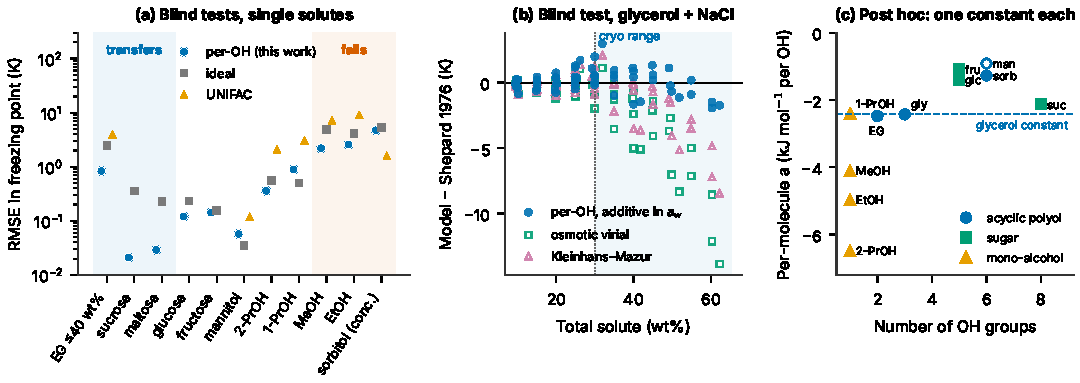
\includegraphics[width=\textwidth]{report_results_v2.pdf}
\caption{(a) Blind tests on single solutes. (b) Glycerol\,+\,NaCl mixtures vs Shepard 1976. (c) Post hoc constants per molecule.}
\end{figure}

\begin{figure}[H]
\centering
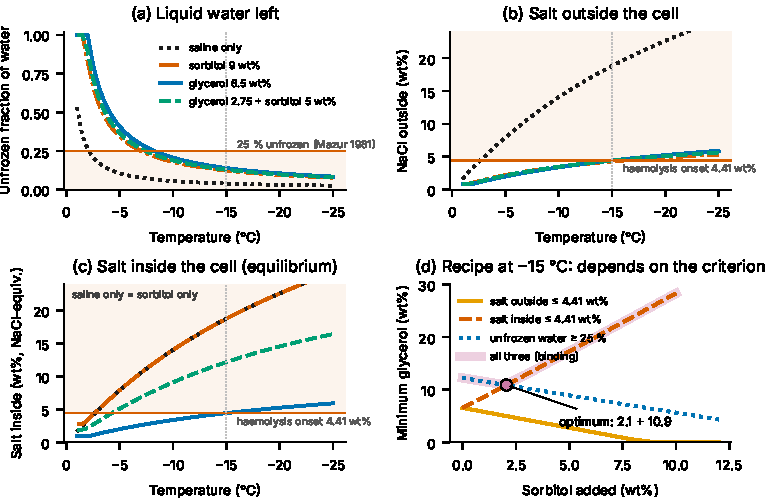
\includegraphics[width=0.9\textwidth]{freeze_concentration_cells.pdf}
\caption{Freeze concentration outside and inside a cell, and recipes under three injury criteria.}
\end{figure}

%======================================================================
\section{The code: what each file does and how to run it}

\subsection{Setup on your laptop}
\begin{enumerate}
\item Install Python 3.10 or newer.
\item Unzip the repository (\file{cryo-sle-full-30oct.zip}) and open a terminal in the \file{cryo-sle} folder.
\item Install the packages: \file{pip install -r requirements.txt}
\item Run the tests: \file{python -m pytest -q} (expect ``14 passed'').
\item Rebuild everything: \file{python run\_all.py} (a few minutes).
\end{enumerate}
\textbf{What you should see from \file{run\_all.py}:} every step marked \texttt{ok}; six prediction files ``reproduces''
and two ``DIFFERS (expected: \ldots)'' with the reason printed; all results tables ``unchanged''; figures written to
\file{figures/}. It runs in a temporary copy, so it can never overwrite a committed prediction.

\textbf{One trap.} Our package is called \file{thermo}, and so is the pip package used for UNIFAC. Always run scripts
from the repository root as \file{python analysis/<name>.py}, never by importing them from elsewhere.

\textbf{Key numbers to check after running} (they should match exactly): $\aoh=-2414.9$ in the first line of
\file{predictions/predictions\_v1.csv}; Shepard RMS 0.69\,K and 1.23\,K in \file{predictions/shepard\_test\_results.csv};
optimum 2.06\,+\,10.86\,wt\% in the last line of \file{predictions/recipe\_three\_criteria.csv}.

\subsection{Repository map}
\begin{xltabular}{\textwidth}{@{}p{5.6cm}L@{}}
\toprule
File & What it does\\
\midrule
\multicolumn{2}{@{}l}{\textbf{Core model (\file{thermo/})}}\\
\file{constants.py} & Water properties ($\dfus H$, $\Delta C_p$, $T_m$) and solute data (molar mass, OH count)\\
\file{composition.py} & Mass fraction $\leftrightarrow$ mole fraction conversions\\
\file{activity.py} & Ideal, Margules and per-OH models: $\ln\gamma_w$ (eq.~\ref{eq:model})\\
\file{sle.py} & Ice equilibrium (eq.~\ref{eq:sle}), freezing point solver, freeze concentration (eq.~\ref{eq:balance})\\
\file{salt.py} & NaCl osmotic coefficient fit; additive salt\,+\,polyol model\\
\file{fit.py} & Least-squares fit, bootstrap, Gibbs--Duhem check\\
\file{optimise.py} & Older recipe optimiser (kept to document the fixed-dose result)\\
\midrule
\multicolumn{2}{@{}l}{\textbf{Fit and predictions (\file{analysis/})}}\\
\file{fit\_literature.py} & Fits $\aoh$ on glycerol; writes the first blind predictions\\
\file{predict\_crc\_extra.py}, \file{predict\_e1.py}, \file{predict\_lab\_set.py}, \file{predict\_salt\_set.py}, \file{predict\_uraji.py} & Blind predictions written before each test's data were seen\\
\midrule
\multicolumn{2}{@{}l}{\textbf{Tests and benchmarks}}\\
\file{check\_literature.py} & Sanity checks on the data file\\
\file{unifac\_compare.py}, \file{plot\_model\_comparison.py} & UNIFAC and Dortmund on glycerol; comparison figure\\
\file{model\_checks.py} & Stability of $\aoh$; one vs two parameters\\
\file{blind\_test\_crc.py}, \file{blind\_test\_e1.py}, \file{blind\_test\_sorbitol\_pg.py} & Single-solute blind tests\\
\file{shepard\_test.py} & Glycerol\,+\,NaCl ternary test\\
\file{sorbitol\_25C.py}, \file{sucrose\_T\_transfer.py} & 25\,\textdegree C tests; temperature vs molecule\\
\file{osmotic\_virial\_benchmark.py} & Cryobiology model benchmark\\
\midrule
\multicolumn{2}{@{}l}{\textbf{Design and application}}\\
\file{glycerol\_sparing.py}, \file{recipe\_sensitivity.py} & Recipe v2 and its sensitivity\\
\file{freeze\_concentration\_cells.py} & Freeze concentration, cell model, three-criteria recipe\\
\file{posthoc\_per\_molecule.py} & Post hoc constants; Gibbs--Helmholtz split\\
\file{run\_recipe.py} & Older recipe demo (superseded)\\
\midrule
\multicolumn{2}{@{}l}{\textbf{Experiment tools}}\\
\file{cooling\_curve.py}, \file{simulate\_curve.py} & Freezing point from a logged cooling curve; synthetic test curves\\
\file{uncertainty\_budget.py} & Uncertainty budget for a measured freezing point\\
\file{arduino/} & DS18B20 logger sketch and serial-to-CSV script\\
\midrule
\multicolumn{2}{@{}l}{\textbf{Outputs and tools}}\\
\file{report\_figures.py} & Report figures from the results files\\
\file{run\_all.py} & Rebuilds everything; checks committed predictions reproduce\\
\file{web/index.html} & Interactive recipe explorer (same model in JavaScript)\\
\file{tests/test\_thermo.py} & 14 unit tests (limits, consistency, solver checks)\\
\file{data/} & Literature data with sources; digitised Shepard data; lab inputs\\
\file{predictions/} & Committed predictions (never edited) and results tables\\
\bottomrule
\end{xltabular}

\subsection{Running one piece at a time}
Any analysis can be run on its own, e.g.\ \file{python analysis/shepard\_test.py} prints its results and writes its
table and figure. The order in \file{run\_all.py} is the order in Section~4.

%======================================================================
\section{Decisions and assumptions (and why)}
\begin{xltabular}{\textwidth}{@{}p{5.2cm}L@{}}
\toprule
Decision & Why\\
\midrule
One parameter, per OH group & Tests whether one physical interaction explains polyol non-ideality; a second parameter was not justified (Section~4.5)\\
Fit on CRC glycerol 2--40\,wt\% only & Best-quality data; below 2\,wt\% rounding dominates\\
Interaction energy independent of $T$ & Simplest assumption, written down before the 25\,\textdegree C test; partly fails (Section~4.12)\\
Additive in $\ln a_w$ for mixtures & Follows from the activity framework; fixed before mixture data\\
Pass mark 0.5\,K for the ternary & Fixed in advance; reported as missed, not changed\\
Salt limit 4.41\,wt\%, design $T=-15$\,\textdegree C & Sourced (Lovelock via Shepard; Gao \& Critser)\\
No toxicity weights & No citable values for sorbitol\\
Cell solutes as isotonic NaCl & Avoids cell-specific parameters; main conclusion does not depend on it\\
Baer 1984 sorbitol excluded & Implies $\phi=1.14$ at infinite dilution, which is impossible\\
\bottomrule
\end{xltabular}

\section{Limitations}
\begin{itemize}
\item Equilibrium only: no cooling-rate kinetics, intracellular ice, glass formation or toxicity.
\item The per-OH constant does not describe six-OH chains or simple alcohols, and is not for room-temperature use.
\item Two sets of test data are digitised from figures (Shepard; Uraji pending), with their own uncertainty.
\item No laboratory measurements yet; the experiment is proposed with predictions committed.
\item UNIFAC numbers come from one library; an independent check (DWSIM) is pending.
\end{itemize}

\section{What is left}
\begin{xltabular}{\textwidth}{@{}p{7.2cm}p{1.6cm}L@{}}
\toprule
Task & Who & Note\\
\midrule
Approve the new headline (sparing depends on injury criterion) & Sid & Blocks submission\\
Read the report and this handbook; mark anything unclear & Sid & Then Q\&A practice\\
Download Uraji 1996 PDF; digitise Fig.~2a & Sid & Predictions already committed\\
Verify Fredenslund 1975 and Weidlich 1987 references & Sid & Google Scholar, 2 min\\
Upload repo to GitHub; add link to the report & Sid & \\
Run \file{run\_all.py} on your laptop; screenshot it & Sid & Evidence you ran it\\
Hostile review in a fresh session & Sid (prompt given) & Before 4 Nov\\
Friend's cold read of the report & Sid & \\
Send last year's reports & Sid & Optional layout match\\
DWSIM UNIFAC check & Sid & Optional\\
Add Uraji results to report; README; Colab notebook & Claude & After the above\\
\bottomrule
\end{xltabular}

\begin{thebibliography}{99}
\small
\bibitem{mazur} P. Mazur, Freezing of living cells: mechanisms and implications, \emph{Am.\ J.\ Physiol.} 247 (1984) C125--C142.
\bibitem{gao} D. Gao, J.\,K. Critser, Mechanisms of cryoinjury in living cells, \emph{ILAR J.} 41 (2000) 187--196.
\bibitem{lovelock10} J.\,E. Lovelock, The haemolysis of human red blood-cells by freezing and thawing, \emph{Biochim.\ Biophys.\ Acta} 10 (1953) 414--426.
\bibitem{lovelock11} J.\,E. Lovelock, The mechanism of the protective action of glycerol against haemolysis by freezing and thawing, \emph{Biochim.\ Biophys.\ Acta} 11 (1953) 28--36.
\bibitem{mazur81} P. Mazur, W.\,F. Rall, N. Rigopoulos, \emph{Biophys.\ J.} 36 (1981) 653--675.
\bibitem{mazur89} P. Mazur, K.\,W. Cole, \emph{Cryobiology} 26 (1989) 1--29.
\bibitem{pegg} D.\,E. Pegg, Principles of cryopreservation, \emph{Methods Mol.\ Biol.} 368 (2007) 39--57.
\bibitem{sandler} S.\,I. Sandler, \emph{Chemical, Biochemical, and Engineering Thermodynamics}, 4th ed., Wiley, 2006.
\bibitem{elliott} J.\,A.\,W. Elliott et al., \emph{J.\ Phys.\ Chem.\ B} 111 (2007) 1775--1785.
\bibitem{zielinski} M.\,W. Zielinski et al., \emph{Cryobiology} 69 (2014) 305--317.
\bibitem{km} F.\,W. Kleinhans, P. Mazur, \emph{Cryobiology} 54 (2007) 212--222.
\bibitem{fahy} G.\,M. Fahy, \emph{Biophys.\ J.} 32 (1980) 837--850.
\bibitem{shepard} M.\,L. Shepard, C.\,S. Goldston, F.\,H. Cocks, \emph{Cryobiology} 13 (1976) 9--23.
\bibitem{zargarzadeh} L. Zargarzadeh, J.\,A.\,W. Elliott, \emph{J.\ Phys.\ Chem.\ B} 123 (2019) 1099--1107.
\bibitem{unifac} Aa. Fredenslund, R.\,L. Jones, J.\,M. Prausnitz, \emph{AIChE J.} 21 (1975) 1086--1099.
\bibitem{dortmund} U. Weidlich, J. Gmehling, \emph{Ind.\ Eng.\ Chem.\ Res.} 26 (1987) 1372--1381.
\bibitem{marcolli} C. Marcolli, Th. Peter, \emph{Atmos.\ Chem.\ Phys.} 5 (2005) 1545--1555.
\bibitem{peres} A.\,M. Peres, E.\,A. Macedo, \emph{Fluid Phase Equilib.} 139 (1997) 47--74.
\bibitem{powellpalm} M.\,J. Powell-Palm, A.\,N. Consiglio, arXiv:2601.12573 (2026).
\bibitem{thermo} C. Bell et al., \emph{thermo} (Python package), v0.6.1.
\bibitem{crc} D.\,R. Lide (ed.), \emph{CRC Handbook of Chemistry and Physics}, Internet Version 2005.
\bibitem{siniti} M. Siniti, S. Jabrane, J.\,M. L\'etoff\'e, \emph{Thermochim.\ Acta} 325 (1999) 171--180.
\bibitem{baer} R.\,J. Baer, K.\,A. Baldwin, \emph{J.\ Dairy Sci.} 67 (1984) 2860--2862.
\bibitem{bower} V.\,E. Bower, R.\,A. Robinson, \emph{J.\ Phys.\ Chem.} 67 (1963) 1540--1541.
\bibitem{robinson} R.\,A. Robinson, R.\,H. Stokes, \emph{Trans.\ Faraday Soc.} 45 (1949) 612--624.
\bibitem{benson} J.\,D. Benson et al., \emph{Cryobiology} 61 (2010) 352--356.
\bibitem{uraji} T. Uraji, H. Kohno, H. Yoshimura, M. Shimoyamada, K. Watanabe, \emph{Food Sci.\ Technol.\ Int.} 2 (1996) 38--42.
\end{thebibliography}

\end{document}
